\subsection{Windows GUI}
Til Windows er der udviklet et view-lag med WPF og C\#. Det findes under namespace "Smartpool.Application.Win."

\subsubsection{Design}
I Windows applikationen designes view-klasser, der implementerer view-interfacet defineret i præsentationslaget.
Designet af Windows GUI er lavet således, at codebehind filerne implementerer hver sit view-interfacet fra præsentationslaget. Codebehind agerer dermed som en bro, i mellem Smartpools præsentationslag, og WPF view-lag.

I klasse diagrammet nedenfor, ses Windows designet, af WinCreateUserView der implementerer ISignUpView fra applikationslaget og har en SignUpViewController.
\begin{figure}
	\centering
	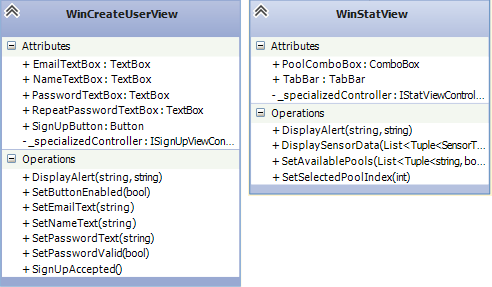
\includegraphics[width=0.7\linewidth]{figs/design/wincreateuserandwinstatviewview}
	\caption{WinCreateUserView og WinStatView}
	\label{fig:wincreateuserandwinstatviewview}
\end{figure}

Ligeledes er view klassen for WinStatView designet.
Klassen ses på figur~\ref{wincreateuserandwinstatviewview}.

For yderligere forklaring se dokumentation afsnit Applikationslaget under Design.